\documentclass[10pt,twocolumn,letterpaper]{article}

\usepackage{cvpr}
\usepackage{times}
\usepackage{epsfig}
\usepackage{graphicx}
\usepackage{amsmath}
\usepackage{amssymb}
\usepackage{breqn}
\usepackage{float}
\usepackage{algorithm}
\usepackage{algorithmic}
\usepackage{amsmath}
\usepackage{capt-of}
\usepackage{pdfpages}
\usepackage{enumerate}
\usepackage{footnote}
\usepackage{multirow}
\usepackage{makecell}
\usepackage{verbatim}

% Include other packages here, before hyperref.

% If you comment hyperref and then uncomment it, you should delete
% egpaper.aux before re-running latex.  (Or just hit 'q' on the first latex
% run, let it finish, and you should be clear).
\usepackage[pagebackref=true,breaklinks=true,letterpaper=true,colorlinks,bookmarks=false]{hyperref}

\cvprfinalcopy % *** Uncomment this line for the final submission

\def\cvprPaperID{3662} % *** Enter the CVPR Paper ID here
\def\httilde{\mbox{\tt\raisebox{-.5ex}{\symbol{126}}}}

% Pages are numbered in submission mode, and unnumbered in camera-ready
\ifcvprfinal\pagestyle{empty}\fi
\begin{document}

%%%%%%%%% TITLE
\title{Supplementary Material for StarGAN: Unified Generative Adversarial Networks \\ for Multi-Domain Image-to-Image Translation}

\onecolumn
\section{Supplementary Material for StarGAN} \label{appendix}
\subsection{Training with Multiple Datasets} 
Fig.\thinspace\ref{figure8} shows an overview of StarGAN when learning from both the CelebA and RaFD datasets. As can be seen at the top of the figure, the label for CelebA contains binary attributes (Black, Blond, Brown, Male, and Young), while the label for RaFD provides information on categorical attributes (Angry, Fearful, Happy, Sad, and Disgusted). The mask vector is a two-dimensional one-hot vector which indicates whether the CelebA or RaFD label is \textit{valid}.


\begin{figure*}[h]
\centering
\centerline{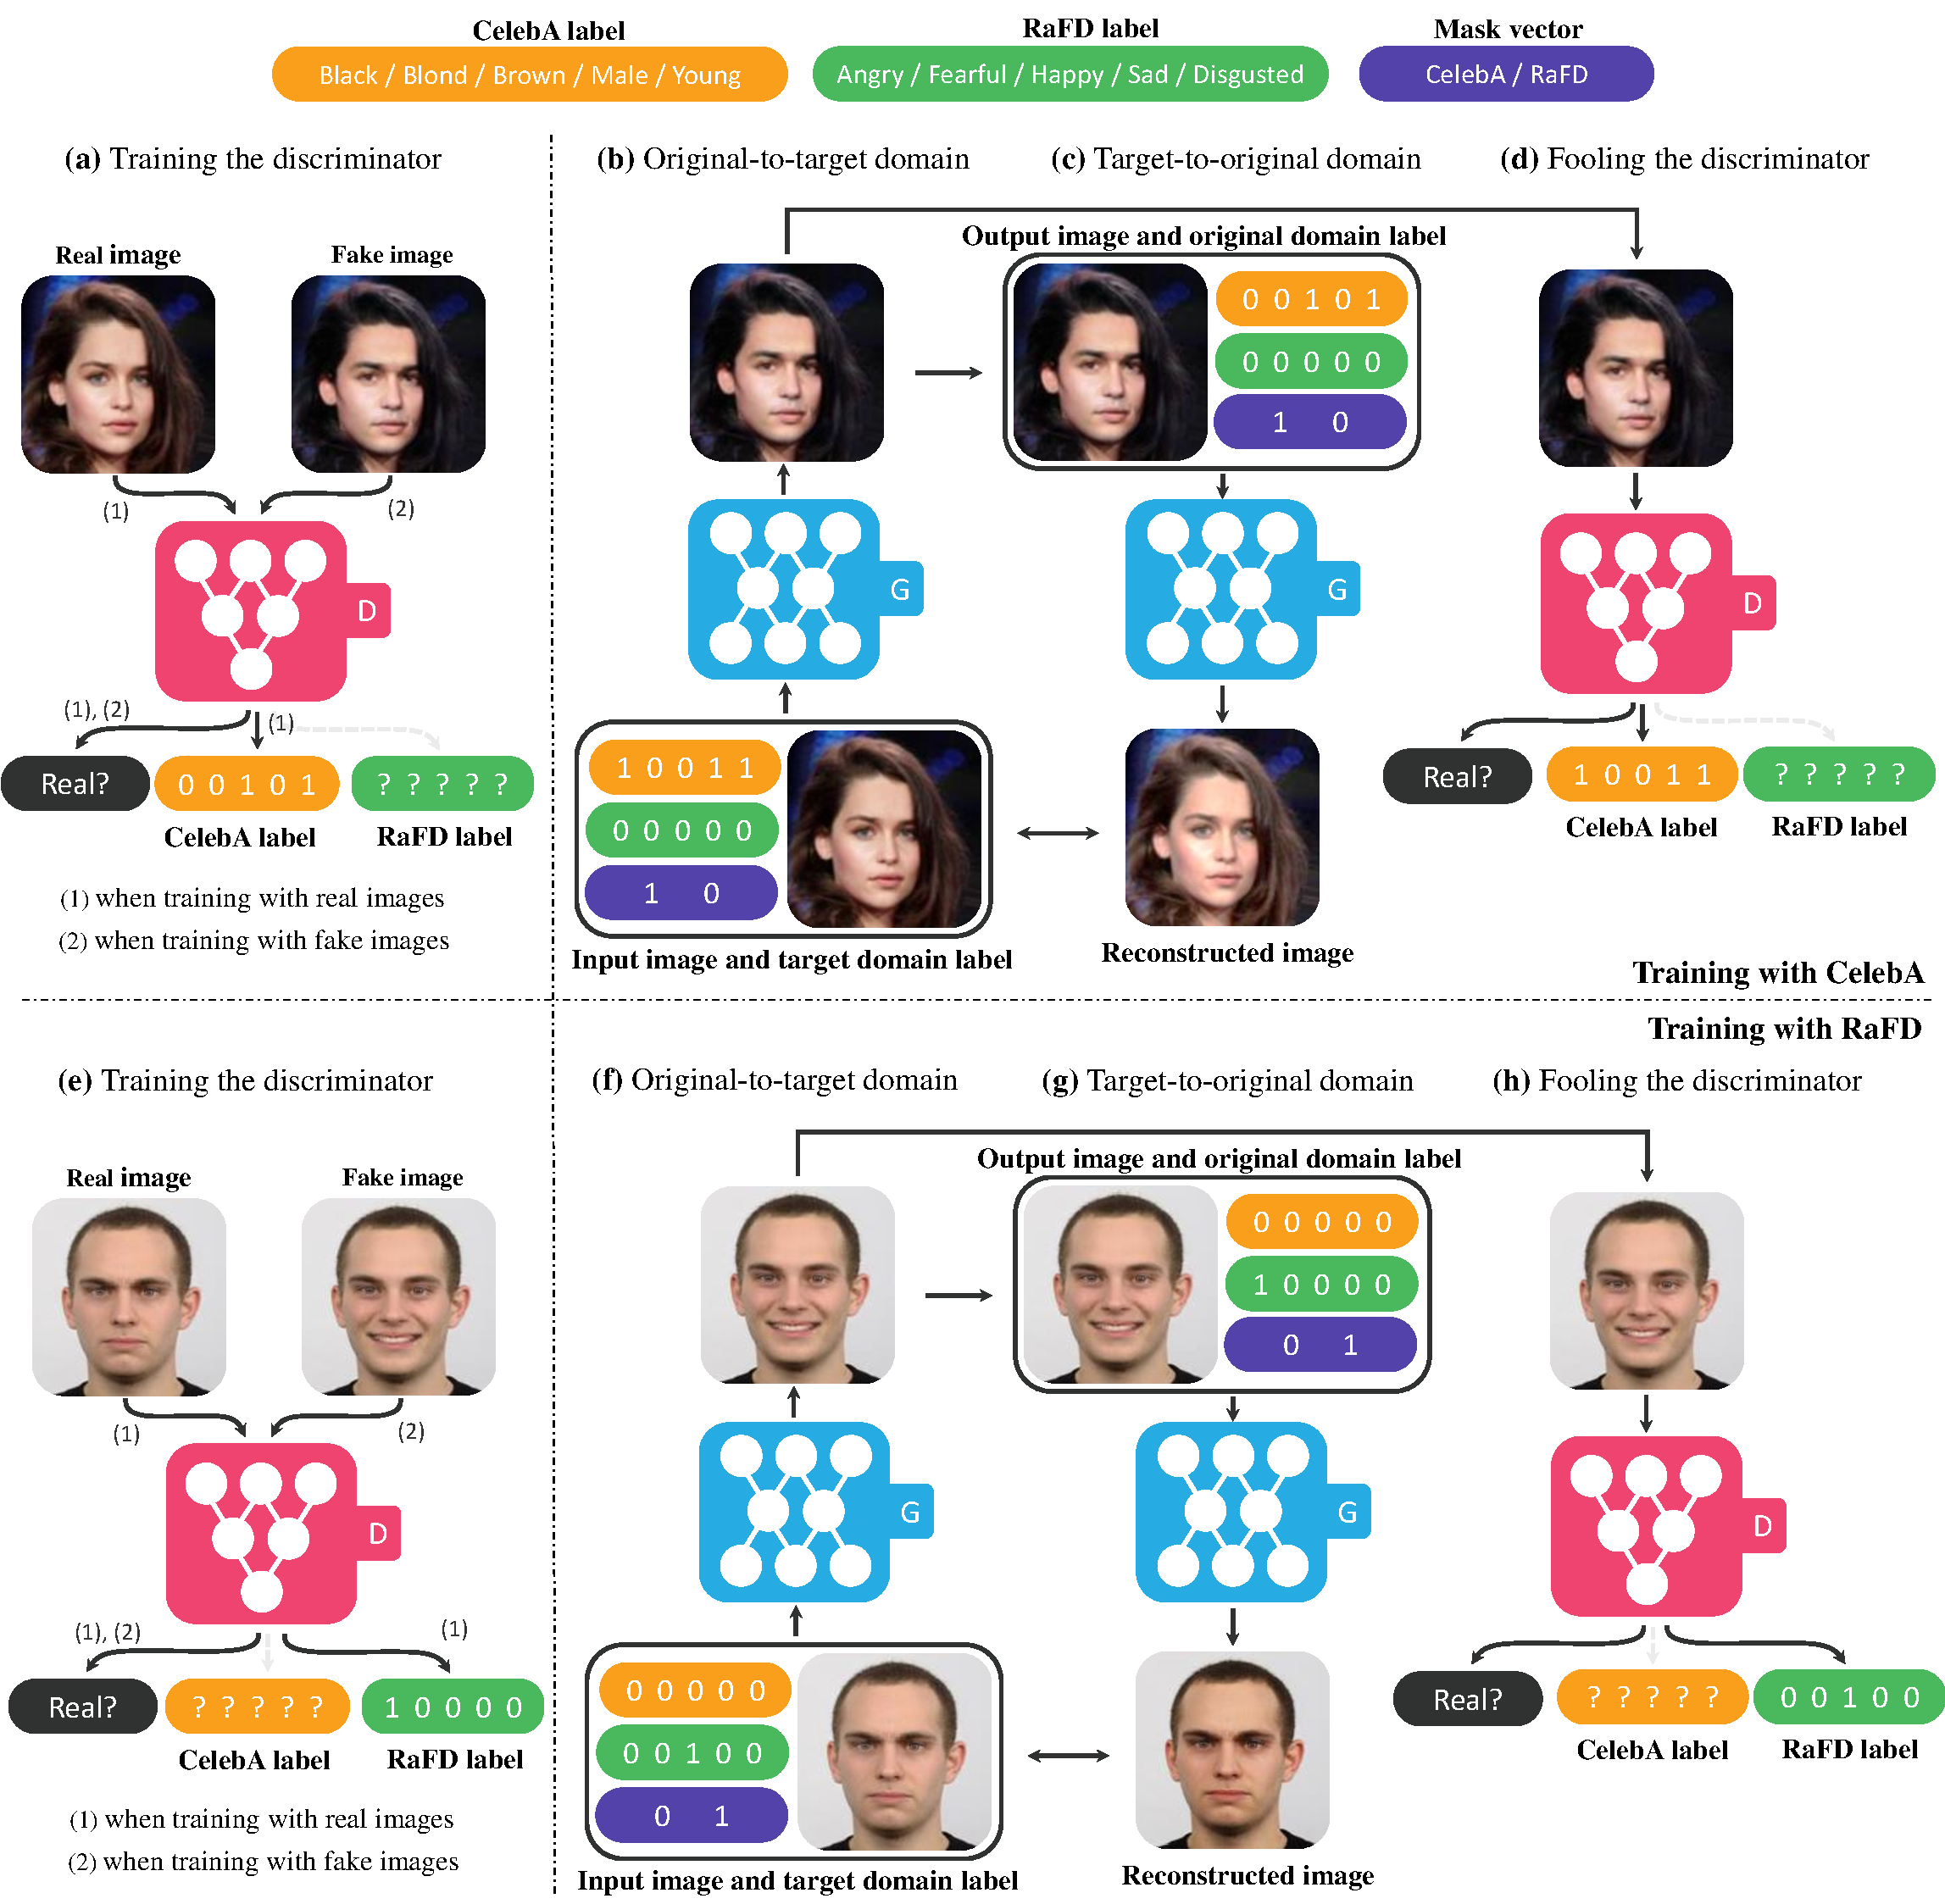
\includegraphics[width=0.95\linewidth]{images/supple_model_final.pdf}}
\medskip
\caption{Overview of StarGAN when training with both CelebA and RaFD. \textbf{(a) $\sim$ (d)} shows the training process using CelebA, and \textbf{(e) $\sim$ (h)} shows the training process using RaFD. \textbf{(a), (e)} The discriminator $D$ learns to distinguish between real and fake images and minimize the classification error only for the known label. \textbf{(b), (c), (f), (g)} When the mask vector (purple) is [1, 0], the generator $G$ learns to focus on the CelebA label (yellow) and ignore the RaFD label (green) to perform image-to-image translation, and vice versa when the mask vector is [0, 1]. \textbf{(d), (h)} $G$ tries to generate images that are both indistinguishable from real images and classifiable by $D$ as belonging to the target domain.}
\label{figure8}
\end{figure*}


\medskip

\subsection{Network Architecture} 
The network architectures of StarGAN are shown in Table \ref{table5} and \ref{table6}.  For the generator network, we use instance normalization in all layers except the last output layer. For the discriminator network, we use Leaky ReLU with a negative slope of 0.01. There are some notations; ${n}_{d}$: the number of domain, ${n}_{c}$: the dimension of domain labels (${n}_{d}+2$ when using a mask vector, otherwise same as ${n}_{d}$), N: the number of output channels, K: kernel size, S: stride size, P: padding size, IN: instance normalization.

\medskip

\begin{comment}

\begin{table*}[h]
\setlength{\tabcolsep}{11pt}
\renewcommand{\arraystretch}{1.3}
\begin{center}
\begin{tabular}{l  l  l  l}
Notation & Description & Notation & Description \\
\hline 
\hline 
$h$ & input image height & $w$ & input image width \\
\hline
${n}_{d}$ & the number of domains & ${n}_{c}$ & the dimension of domain labels (${n}_{d}$ or ${n}_{d} + 2$)\\ 
\hline
CONV & convolution & DECONV & transposed convolution\\
\hline 
FC & fully connected & IN & instance normalization \\
\hline
N & the number of output channels & K & kernel size \\
\hline 
S & stride size & P & padding size \\
\hline\hline 
\end{tabular}
\end{center}
\caption{Notations in the Table\thinspace\ref{table5} and \ref{table6}}
\end{table*}

\end{comment}


\begin{table*}[h]
\setlength{\tabcolsep}{13pt}
\renewcommand{\arraystretch}{1.7}
\begin{center}
\begin{tabular}{c  c  c}
Part & Input $\rightarrow$ Output Shape & Layer Information \\
\hline \hline
\multirow{3}{*}{Down-sampling} & $(h, w, 3+{n}_{c}) \rightarrow (h, w, 64)$ & CONV-(N64, K7x7, S1, P3), IN, ReLU \\
& $(h, w, 64) \rightarrow (\frac{h}{2}, \frac{w}{2}, 128)$ & CONV-(N128, K4x4, S2, P1), IN, ReLU \\
& $(\frac{h}{2}, \frac{w}{2}, 128) \rightarrow (\frac{h}{4}, \frac{w}{4},256)$ & CONV-(N256, K4x4, S2, P1), IN, ReLU \\
\Xhline{1.0pt}
\multirow{6}{*}{Bottleneck} & $(\frac{h}{4}, \frac{w}{4}, 256) \rightarrow (\frac{h}{4}, \frac{w}{4}, 256)$ & Residual Block: CONV-(N256, K3x3, S1, P1), IN, ReLU\\
 & $(\frac{h}{4}, \frac{w}{4}, 256) \rightarrow (\frac{h}{4}, \frac{w}{4}, 256)$ &  Residual Block: CONV-(N256, K3x3, S1, P1), IN, ReLU \\
 & $(\frac{h}{4}, \frac{w}{4}, 256) \rightarrow (\frac{h}{4}, \frac{w}{4}, 256)$ &   Residual Block: CONV-(N256, K3x3, S1, P1), IN, ReLU  \\
 & $(\frac{h}{4}, \frac{w}{4}, 256) \rightarrow (\frac{h}{4}, \frac{w}{4}, 256)$ &   Residual Block: CONV-(N256, K3x3, S1, P1), IN, ReLU  \\
 & $(\frac{h}{4}, \frac{w}{4}, 256) \rightarrow (\frac{h}{4}, \frac{w}{4}, 256)$ &   Residual Block: CONV-(N256, K3x3, S1, P1), IN, ReLU  \\
 & $(\frac{h}{4}, \frac{w}{4}, 256) \rightarrow (\frac{h}{4}, \frac{w}{4}, 256)$ &   Residual Block: CONV-(N256, K3x3, S1, P1), IN, ReLU  \\
\Xhline{1.0pt}
\multirow{3}{*}{Up-sampling} & $(\frac{h}{4}, \frac{w}{4}, 256) \rightarrow (\frac{h}{2}, \frac{w}{2}, 128)$ & DECONV-(N128, K4x4, S2, P1), IN, ReLU \\
 & $(\frac{h}{2}, \frac{w}{2}, 128) \rightarrow (h, w, 64)$ & DECONV-(N64, K4x4, S2, P1), IN, ReLU \\
 & $(h, w, 64) \rightarrow (h, w, 3)$ & CONV-(N3, K7x7, S1, P3), Tanh \\
\hline
\hline
\end{tabular}
\end{center}
\caption{Generator network architecture}
\label{table5}
\end{table*}

\medskip

\begin{table*}[h]
\setlength{\tabcolsep}{15pt}
\renewcommand{\arraystretch}{1.7}
\begin{center}
\begin{tabular}{c c c}
Layer & Input $\rightarrow$ Output Shape & Layer Information \\
\hline \hline
Input Layer & $(h, w, 3) \rightarrow (\frac{h}{2}, \frac{w}{2}, 64) $ & CONV-(N64, K4x4, S2, P1), Leaky ReLU \\
\Xhline{1.0pt}
Hidden Layer & $(\frac{h}{2}, \frac{w}{2}, 64) \rightarrow (\frac{h}{4}, \frac{w}{4}, 128) $ & CONV-(N128, K4x4, S2, P1), Leaky ReLU \\
Hidden Layer & $(\frac{h}{4}, \frac{w}{4}, 128) \rightarrow (\frac{h}{8}, \frac{w}{8}, 256) $ & CONV-(N256, K4x4, S2, P1), Leaky ReLU \\
Hidden Layer & $(\frac{h}{8}, \frac{w}{8}, 256) \rightarrow (\frac{h}{16}, \frac{w}{16}, 512) $ & CONV-(N512, K4x4, S2, P1), Leaky ReLU \\
Hidden Layer & $(\frac{h}{16}, \frac{w}{16}, 512) \rightarrow (\frac{h}{32}, \frac{w}{32}, 1024) $ & CONV-(N1024, K4x4, S2, P1), Leaky ReLU \\
Hidden Layer & $(\frac{h}{32}, \frac{w}{32}, 1024) \rightarrow (\frac{h}{64}, \frac{w}{64}, 2048) $ & CONV-(N2048, K4x4, S2, P1), Leaky ReLU \\
\Xhline{1.0pt}
Output Layer (${D}_{src}$) & $(\frac{h}{64}, \frac{w}{64}, 2048) \rightarrow (\frac{h}{64}, \frac{w}{64}, 1) $ & CONV-(N1, K3x3, S1, P1) \\
Output Layer (${D}_{cls}$) & $(\frac{h}{64}, \frac{w}{64}, 2048) \rightarrow (1, 1, {n}_{d}) $ & CONV-(N(${n}_{d}$), K$\frac{h}{64}$x$\frac{w}{64}$, S1, P0) \\
\hline \hline
\end{tabular}
\end{center}
\caption{Discriminator network architecture}
\label{table6}
\end{table*}

\medskip
\subsection{Additional Qualitative Results} 
Figs. \ref{figure9}, \ref{figure10}, \ref{figure11}, and \ref{figure12} show additional images with $256 \times 256$ resolutions generated by StarGAN. All images were generated by a single generator trained on both the CelebA and RaFD datasets. We trained StarGAN on a single NVIDIA Pascal M40 GPU for seven days.
\begin{figure*}[h]
\centering
\centerline{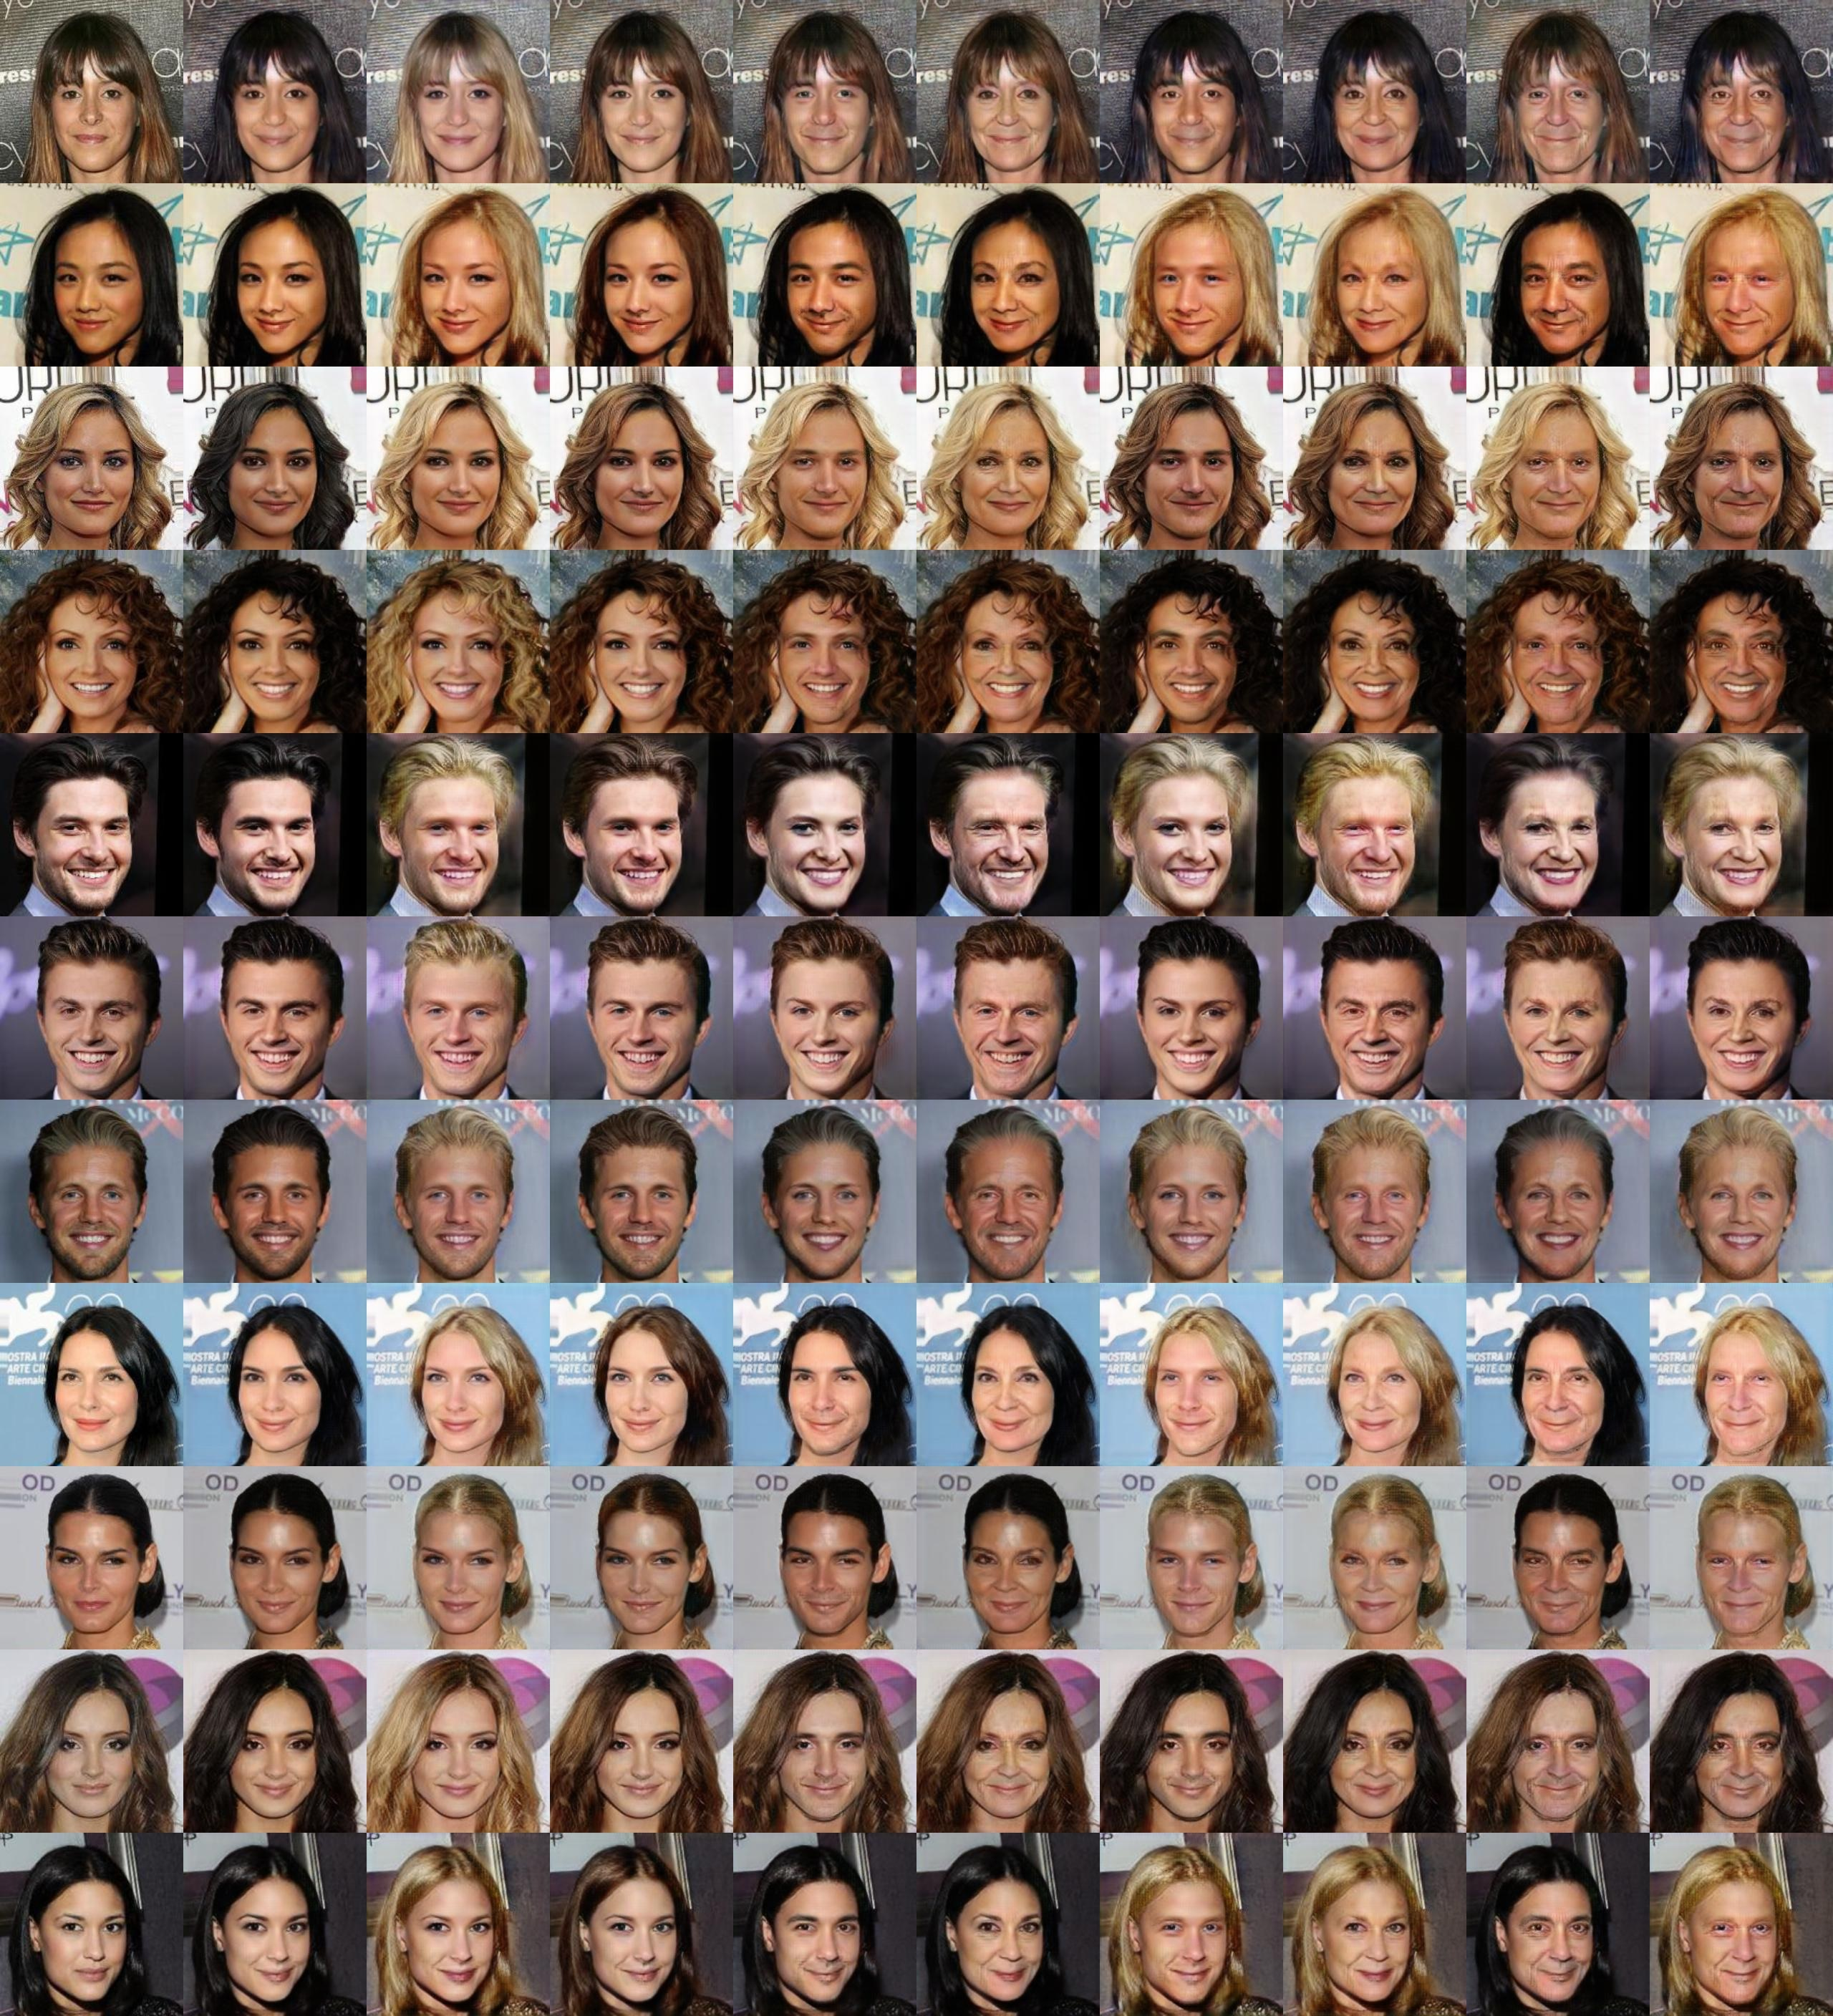
\includegraphics[width=1.0\linewidth]{images/supple_CelebA_single_multi.jpg}}
\caption{Single and multiple attribute transfer on CelebA (Input, Black hair, Blond hair, Brown hair, Gender, Aged, Hair color + Gender, Hair color + Aged, Gender + Aged, Hair color + Gender + Aged).}
\label{figure9}
\end{figure*}

\begin{figure*}[t]
\centering
\centerline{\includegraphics[width=1.0\linewidth]{images/supple_CelebA_attr_8.jpg}}
\caption{Single attribute transfer on CelebA (Input, Black hair, Blond hair, Brown hair, Gender, Mouth, Pale skin, Rose cheek, Aged).}
\label{figure10}
\end{figure*}

\begin{figure*}[t]
\centering
\centerline{\includegraphics[width=1.0\linewidth]{images/supple_rafd2.jpg}}
\caption{Emotional expression synthesis on RaFD (Input, Angry, Contemptuous, Disgusted, Fearful, Happy, Neutral, Sad, Surprised ).}
\label{figure11}
\end{figure*}

\begin{figure*}[h]
\centering
\centerline{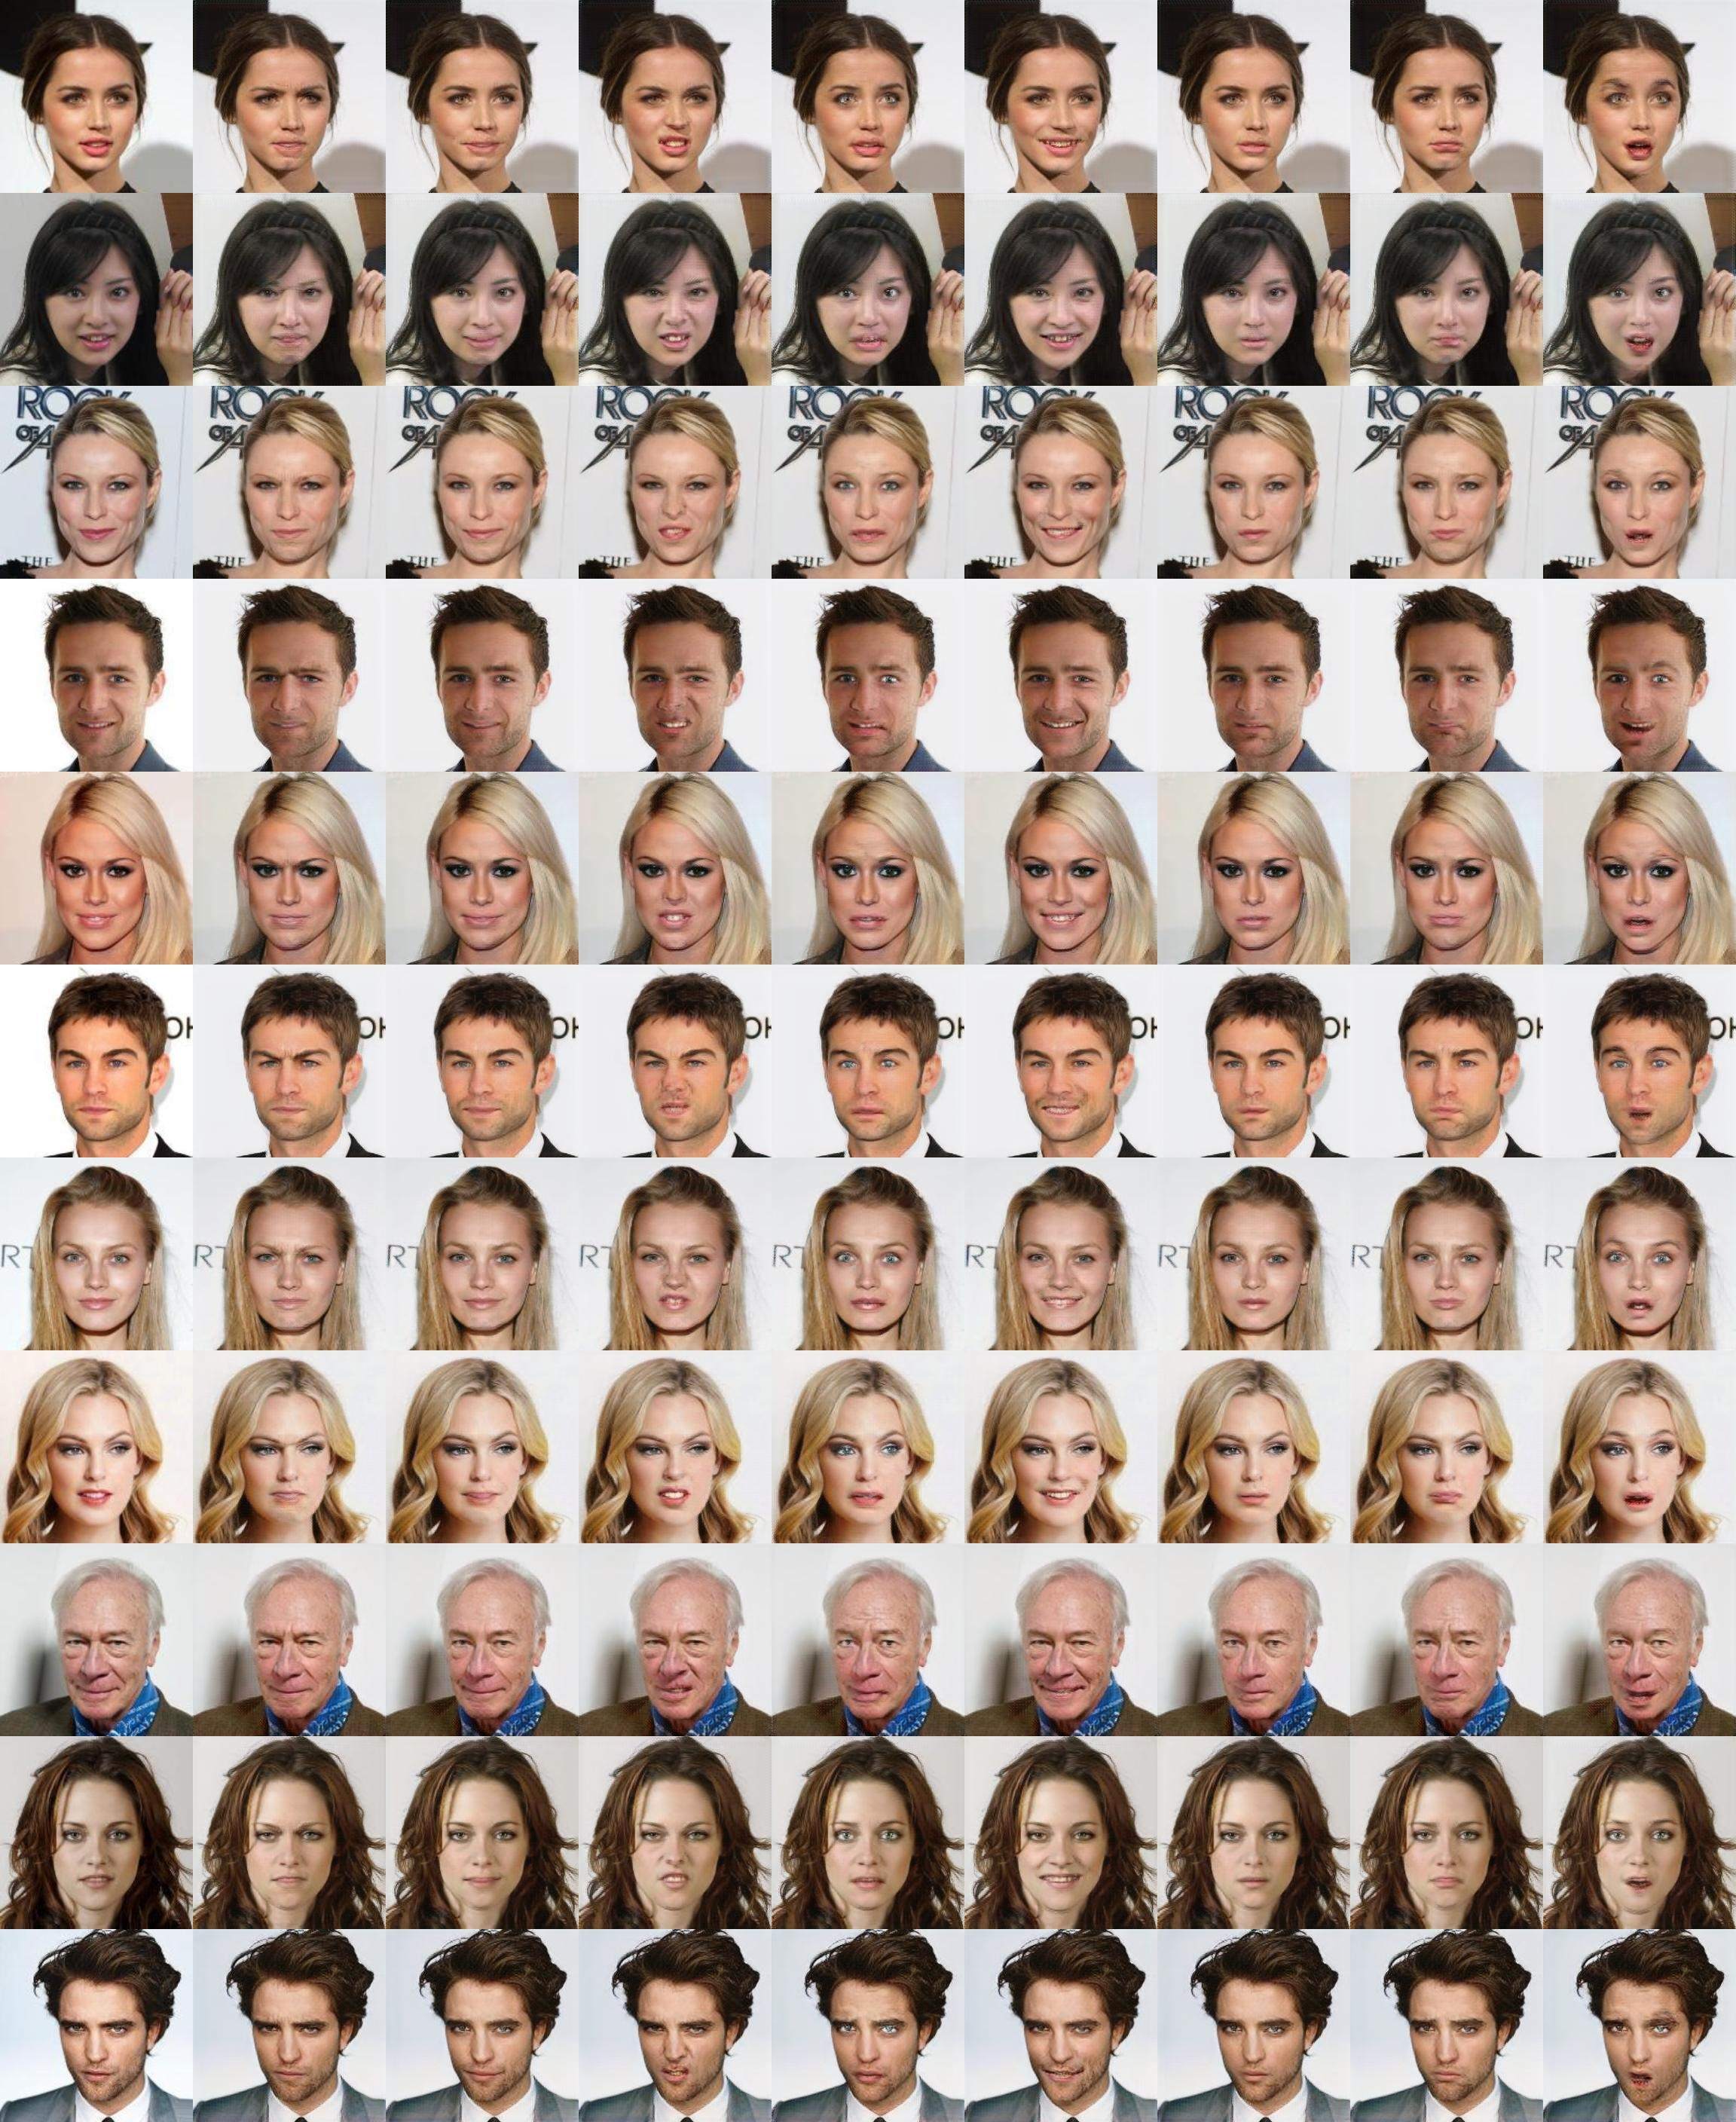
\includegraphics[width=1.0\linewidth]{images/supple_CelebA_expr.jpg}}
\caption{Emotional expression synthesis on CelebA (Input, Angry, Contemptuous, Disgusted, Fearful, Happy, Neutral, Sad, Surprised).}
\label{figure12}
\end{figure*}

\end{document}
